% Copyright (C) 2012 Shi.Zhan <g.shizhan.g@gmail.com>
%
% Permission is hereby granted, free of charge, to any person obtaining a copy of this software and associated documentation files (the "Software"), to deal in the Software without restriction, including without limitation the rights to use, copy, modify, merge, publish, distribute, sublicense, and/or sell copies of the Software, and to permit persons to whom the Software is furnished to do so, subject to the following conditions:
%
% The above copyright notice and this permission notice shall be included in all copies or substantial portions of the Software.
%
% THE SOFTWARE IS PROVIDED "AS IS", WITHOUT WARRANTY OF ANY KIND, EXPRESS OR IMPLIED, INCLUDING BUT NOT LIMITED TO THE WARRANTIES OF MERCHANTABILITY, FITNESS FOR A PARTICULAR PURPOSE AND NONINFRINGEMENT. IN NO EVENT SHALL THE AUTHORS OR COPYRIGHT HOLDERS BE LIABLE FOR ANY CLAIM, DAMAGES OR OTHER LIABILITY, WHETHER IN AN ACTION OF CONTRACT, TORT OR OTHERWISE, ARISING FROM, OUT OF OR IN CONNECTION WITH THE SOFTWARE OR THE USE OR OTHER DEALINGS IN THE SOFTWARE.
%
% 课程:人机交互技术及应用
% 班级:传播学1001班
% 课时:40学时,2012年秋季1~10周,每周一、三
% 地点:东九楼D212
% 主页:http://code.google.com/p/hci-course/
% 教师:施展 
% 单位:华中科技大学 武汉光电国家实验室
%
\documentclass{beamer}
\usepackage{fontspec,xunicode,xltxtra,beamerthemesplit}
%\usetheme{Hannover} % White background
\usetheme{Berkeley} % Blue background
\setmainfont[
	BoldFont={WenQuanYi Zen Hei},
	ItalicFont={WenQuanYi Micro Hei}
]{WenQuanYi Micro Hei}
\setsansfont[
	BoldFont={WenQuanYi Zen Hei},
	ItalicFont={WenQuanYi Micro Hei}
]{WenQuanYi Micro Hei}

% 中文环境自动换行
\XeTeXlinebreaklocale "zh"
\XeTeXlinebreakskip = 0pt plus 1pt

% 中文环境修正导航栏
\makeatletter
\def\beamer@linkspace#1{
	\begin{pgfpicture}{0pt}{-1.5pt}{#1}{5.5pt}
		\pgfsetfillopacity{0}
		\pgftext[x=0pt,y=-1.5pt]{.}
		\pgftext[x=#1,y=5.5pt]{.}
	\end{pgfpicture}
}
\makeatother

% diagrams
\usepackage{tikz}
\usetikzlibrary{arrows,shapes}

% full page image
\newcommand{\fullPageImage}[2]{
	{
		\usebackgroundtemplate{\includegraphics[width=\paperwidth, height=\paperheight]{#1}}
		\frame[plain]{#2}
	}
}

\title{人机交互技术}
\author{施展}
\institute{华中科技大学~武汉光电国家实验室}
\date{\today}
\titlegraphic{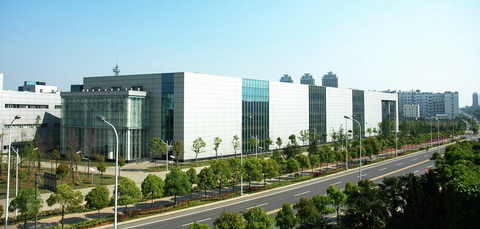
\includegraphics[width=2cm]{images/wnlo.jpg}}

\begin{document}

\begin{frame}
	\titlepage
\end{frame}

\begin{frame}
	\frametitle{内容提要}
	\tableofcontents
\end{frame}

\section{第四讲}
\begin{frame}
	\frametitle{第四讲 交互技术}
	\begin{itemize}
		\item 人机交互输入模式
		\item 基本交互技术
		\item 图形交互技术
		\item 语音交互技术
		%\item 笔交互技术
	\end{itemize}
\end{frame}

\subsection{人机交互输入模式}
\begin{frame}
	\frametitle{人机交互输入模式}
	\beamertemplatetransparentcovereddynamicmedium
	\begin{itemize}[<+->]
		\item 输入设备多种多样;
		\item 对一个应用程序而言,可以有多个输入设备,同一个设备又可能为多个任务服务;
		\item 要求对输入过程的处理要有合理的模式。
		\begin{itemize}
			\item 请求模式 (Request Mode)
			\item 采样模式 (Sample Mode)
			\item 事件模式 (Event Mode)
		\end{itemize}
	\end{itemize}
\end{frame}

\subsection{基本交互技术}
\begin{frame}
	\frametitle{基本交互技术}
	\beamertemplatetransparentcovereddynamicmedium
	\tikzstyle{block} = [
		rectangle,
		rounded corners,
		draw=black, very thick,
		fill=blue!20,
		text width=8em,
		minimum height=2em,
		text centered]
	\tikzstyle{line} = [
		draw, -latex',
		draw=black, very thick,
		text centered]

	\begin{columns}
		\column{.5\textwidth}
		\begin{itemize}
			\item 请求模式~{\tiny 应用程序驱动设备}
			\begin{itemize}
				\item 在请求模式下,由应用程序负责启动输入设备。
				\item 应用程序执行过程中需要输入数据时,暂停程序的执行,直到从输入设备接受到请求的输入数据后,才继续执行程序。
			\end{itemize}
		\end{itemize}
		\column{.5\textwidth}
		\begin{center}
		\begin{tikzpicture}[node distance=1.5cm, auto,]
		    \node [block] (init) {程序工作,输入设备等待程序请求};\pause
		    \node [block, below of=init] (cmd) {收到请求指令};
		    \path [line] (init) -- (cmd);\pause
		    \node [block, below of=cmd] (data) {输入设备工作,程序等待接收数据};
		    \path [line] (cmd) -- (data);\pause
		    \node [block, below of=data] (done) {请求完成}
		    	edge[line, bend right=60] (init.east);
		    \path [line] (data) -- (done);
		\end{tikzpicture}
		\end{center}
	\end{columns}
\end{frame}

\begin{frame}
	\frametitle{基本交互技术}
	\beamertemplatetransparentcovereddynamicmedium
	\tikzstyle{block} = [
		rectangle,
		rounded corners,
		draw=black, very thick,
		fill=blue!20,
		text width=6em,
		minimum height=2em,
		text centered]
	\tikzstyle{line} = [
		draw, -latex',
		draw=black, very thick,
		text centered]

	\begin{itemize}
		\item 采样模式~{\tiny 输入设备和应用程序相互独立}
		\begin{itemize}
			% 输入设备连续不断地把信息输入进来,信息的输入和应用程序中的输入命令无关。
			% 应用程序在处理其它数据的同时,输入设备也在工作,新的输入数据替换以前的输入数据。
			% 当应用程序遇到取样命令时,读取当前保存的输入设备数据。
			\item 优点:这种模式对连续的信息流输入比较方便,也可同时处理多个输入设备的输入信息。
			\item 缺点:应用处理滞后,可能丢失信息。
		\end{itemize}
	\end{itemize}
	\begin{center}
	\begin{tikzpicture}[node distance=1.5cm, auto,]
	    \node [] (center) {};\pause
	    \node [block, right of=center] (device) {输入设备工作};\pause
	    \node [block, below of=device] (data) {数据生成}
	    	edge[line, bend right=60] (device.east);
	    \path [line] (device) -- (data);\pause
	    \node [block, below of=center, left of=data] (buffer) {数据缓存区};
	    \path [line] (data) -- (buffer);\pause
	    \node [block, left of=center] (program) {程序工作};\pause
	    \node [block, below of=program] (sample) {数据采样}
	    	edge[line, bend left=60] (program.west);
	    \path [line] (program) -- (sample);
	    \path [line] (buffer) -- (sample);
	\end{tikzpicture}
	\end{center}
\end{frame}

\begin{frame}
	\frametitle{基本交互技术}
	\beamertemplatetransparentcovereddynamicmedium
	\tikzstyle{block} = [
		rectangle,
		rounded corners,
		draw=black, very thick,
		fill=blue!20,
		text width=2em,
		minimum height=2em,
		text centered]
	\tikzstyle{queue} = [
		draw, rectangle split,
		rectangle split parts=5, minimum width=1cm, minimum height=0.5cm]
	\tikzstyle{line} = [
		draw, -latex',
		draw=black, very thick,
		text centered]

	\begin{itemize}
		\item 事件模式~{\tiny 输入设备和程序并行工作}
		\begin{itemize}
			\item 输入设备把数据保存到一个输入队列,也称为事件队列,所有的输入数据都保存起来,不会遗失。
			\item 应用程序随时可以检查这个事件队列,处理队列中的事件,或删除队列中的事件。
		\end{itemize}
	\end{itemize}
	\begin{center}
	\begin{tikzpicture}[node distance=1.5cm, auto,]
		\node [] (device) {输入};\pause
		\node [queue, below of=device, right of=device] (R){
			\nodepart{two} \nodepart{three}事件
			\nodepart{four} \nodepart{five}
		};
		\draw [line] (device.east) -| (R.north);\pause
		\node [block, below of=R, right of=R] (poll) {检查};
		\draw [line] (R.south) |- (poll.west);\pause
		\node [block, right of=poll] (handlerA) {{\tiny 事件A处理}};
		\draw [line] (poll.east) -- (handlerA.west);
		\node [block, above of=handlerA] (handlerB) {{\tiny 事件B处理}};
		\draw [line] (poll.east) -- (handlerB.west);
		\node [block, above of=handlerB] (handlerC) {{\tiny 事件C处理}};
		\draw [line] (poll.east) -- (handlerC.west);
	\end{tikzpicture}
	\end{center}
\end{frame}

\begin{frame}
	\frametitle{C10K问题}
	% http://blog.csdn.net/ciaos/article/details/7774209
	\begin{center}
	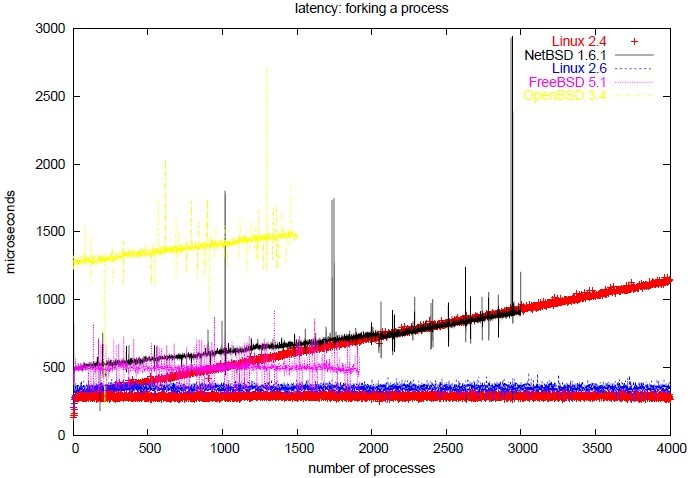
\includegraphics[width=.7\textwidth]{images/c10K.jpg} 
	\end{center}
	\begin{itemize}
	\item 海量用户并发访问显著影响着Web应用服务用户体验
	\end{itemize}
\end{frame}

% http://biancheng.dnbcw.info/python/348697.html
\fullPageImage{images/socket.jpg}{\transwipe}
\fullPageImage{images/epoll.jpg}{\transwipe}
\fullPageImage{images/tornado.jpg}{\transwipe}

\subsection{图形交互技术}
\begin{frame}
	\frametitle{图形交互技术}

\end{frame}

\subsection{语音交互技术}
\begin{frame}
	\frametitle{语音交互技术}

\end{frame}

%\subsection{笔交互技术}
%\begin{frame}
%	\frametitle{笔交互技术}
%
%\end{frame}

\section{小结}
\begin{frame}
	\frametitle{小结}
	\begin{itemize}
		\item 理解人机交互输入模式
		\item 了解主要交互技术
	\end{itemize}
\end{frame}
 
\begin{frame}
	\frametitle{参考文献}
	\bibliographystyle{plain}
	\bibliography{hci}
\end{frame}

\end{document}